\documentclass[iop,twocolappendix]{emulateapj}
\usepackage{blindtext}
%\usepackage{float}
\usepackage{placeins}
\usepackage{graphicx}
\usepackage{amssymb, amsmath}
\usepackage{natbib}
\usepackage{amsmath}
\usepackage{bm}
\usepackage{color}
\usepackage[colorlinks,urlcolor=blue,citecolor=blue,linkcolor=blue]{hyperref}
%\usepackage{subfigure}
%\usepackage{caption}
%\usepackage{subcaption}
\interfootnotelinepenalty=10000
\usepackage[caption=false]{subfig}
\DeclareMathOperator{\sech}{sech}
\begin{document}
\title{The Mechanism of Electron Acceleration in trans-relativistic magnetic reconnection}

\author{David Ball,\altaffilmark{1,3} Lorenzo Sironi,\altaffilmark{2} and Feryal \"Ozel\altaffilmark{1}}

\altaffiltext{1}{Department of Astronomy and Steward Observatory, Univ. of Arizona, 933 N. Cherry Avenue, Tucson, AZ 85721, USA}

\altaffiltext{2}{Department of Astronomy, Columbia University, 550 West 120th Street, New York, NY 10027, USA}
\altaffiltext{3}{Email: davidrball@email.arizona.edu}

\begin{abstract}
We investigate electron acceleration mechanisms in a trans-relativistic low-$\beta$ electron-proton plasma.  By varying the guide field and whether or not we trigger reconnection, we vary the number of x-points and plasmoids that form in a given simulation, which we show plays an important role in particle acceleration.  Using acceleration diagnostics that are calculated on-the-fly for all of the particles in the simulation, we show that x-points, either in the primary current layer or in between merging plasmoids are a necessary first step to accelerate electrons out of the cold initial distribution to highly relativistic ($\gamma > 300$) energies.  Once an electron goes through this step, it can be further accelerated by different mechanisms that may be energetically dominant compared to the initial acceleration at an x-point, but the vast majority of the highly relativistic ($\gamma > 1000$) electrons across our simulations are first accelerated at an x-point.  We show a strong correlation between the work done by the out-of-plane component of electric fields that are parallel to the local magnetic field and the final energy of the particles, emphasizing the importance of the non-ideal field at x-points.  We also include populations of test particles that only feel certain components of the parallel electric field and show that the out-of-plane component of parallel electric fields associated with x-points is responsible for generating a high-energy power-law tail, while the in-plane components are associated with bulk heating.


%Specifically, when no guide field is present, the secondary tearing mode is active and forms copious x-points and plasmoids.  X-points directly accelerate particles through a strong non-ideal field, while plasmoids merge and form current sheets in between them, which serve as sites of further acceleration. When less x-points and plasmoids form, either by suppressing the secondary tearing mode, o

%We further emphasize the effect of varying the number of x-points by comparing triggered and untriggered simulations. In an untriggered simulation there are more x-points and plasmoids than a triggered simulation with identical physical parameters.  Indeed, we find that the spectra from untriggered simulations are systematically harder than their triggered counterparts due to the increased number of x-points and plasmoid mergers.

\end{abstract}
\keywords{magnetic reconnection --- accretion, accretion disks ---galaxies: jets ---X-rays: binaries --- radiation mechanisms: nonthermal --- acceleration of particles} 
\maketitle

\section{introduction} \label{introduction}
Magnetic reconnection is thought to play an important role in accelerating electrons and powering high-energy emission in numerous astrophysical systems including blazar jets (\citealt{giannios2013}; \citealt{petropoulou2016}; \citealt{nalewajko2016}), pulsar wind nebulae (\citealt{coroniti1990}; \citealt{lyubarsky2001}; \citealt{zenitani2001}; \citealt{kirk2003}; \citealt{contopoulos2007}; \citealt{petri2008}; \citealt{sironi2011}; \citealt{cerutti2012, cerutti2014}; \citealt{cerutti2017}; \citealt{philippov2014}), gamma ray bursts (\citealt{thompson1994, thompson2006}; \citealt{usov1994}; \citealt{spruit2001}; \citealt{drenkhahn2002}; \citealt{lyutikov2003}; \citealt{giannios2008}), the Sun (\citealt{forbes1996}; \citealt{yokoyama2001}; \citealt{shibata2011}), and accretion flows around black holes (\citealt{galeev1979}; \citealt{dimatteo1998}; \citealt{uzdensky2008}; \citealt{li2015}; \citealt{ball2016, ball2017}; \citealt{li2017}; \citealt{dalpino2018}; \citealt{ramirez2018}).  Despite its ubiquity, the physics of particle acceleration through reconnection is not fully understood.  

Numerous studies have investigated electron acceleration mechanisms in both relativistic (\citealt{nalewajko2015}; \citealt{guo2015}; \citealt{werner2017}) and nonrelativistic reconnection (\citealt{dahlin2014}; \citealt{li_guo_2017}; \citealt{wangh2016}).  These studies generally take one of two approaches: some apply a guiding center formalism (e.g., \citealt{dahlin2014}) in which they can cleanly separate different acceleration mechanisms in the energy equation for a single particle and ultimately assess the various contributions solely by looking at cell averaged currents, velocities,  and fields. However, this formalism breaks down at x-points in anti-parallel reconnection, where the magnetic field vanishes.  Others look at individual particle trajectories to assess where and by what mechanisms particles are being accelerated.  However, these studies have so far sparsely sampled a collection of representative particles.  Furthermore, most of these studies employ either a pair-plasma or a significantly reduced mass ratio. 

These previous studies have highlighted a few distinct acceleration mechanisms.  One such mechanism is acceleration by the out-of-plane (i.e., in the direction of $\vec{\nabla} \times \vec{B}$) electric field at x-points (citations).  These x-points can occur not only in the in the initial current sheet via the primary or secondary tearing mode, but also in the current sheets generated between merging plasmoids, where reconnection also occurs.  Another prominent mechanism is Fermi reflection, enabled by the various macro-scale motions induced by reconnection.  Fermi reflection can occur between merging plasmoids (citations), within contracting plasmoids (citations), and also between outflows and plasmoids (citations).  \citet{nalewajko2015} also found that particles are accelerated in the trailing edges of plasmoids as they move.

In \citet{ball2018} we investigated particle acceleration in the trans-relativistic regime and found preliminary evidence for the role of x-points, plasmoids, and Fermi-type processes by examining the histories of a few representative high-energy particles.  We did not, however, examine a statistically meaningful sample of particles.  In that study, we observed that at low-$\beta$, electron acceleration is characterized by extremely short periods of intense acceleration by a non-ideal electric field at x-points in the initial sheet or between merging plasmoids.  In contrast, at high-$\beta$ when electrons start out relativistic, x-point acceleration is negligible, and Fermi reflection dominates.  The reason for this is twofold; first, the secondary tearing mode is suppressed at high-$\beta$; second, the energy gain via Fermi reflection off of features moving at the Alfv\'en speed dominates over the energy gain at x-points when the particles already have relativistic velocities.

In this paper, we investigate the physical mechanisms of electron acceleration by comparing four simulations in which we vary the number of x-points and plasmoids by changing guide field strength and whether or not we trigger reconnection.  We address the issues of downsampling in time and particle number, as well as the reduced mass ratio by performing simulations with the realistic electron-proton mass ratio while including particle acceleration diagnostics that are calculated on-the-fly during the simulation for all of the particles.  We also employ robust methods of identifying x-points and track the role of the work done parallel to the local magnetic field in order to investigate the detailed histories of the accelerated particles.  

We find that x-points and plasmoid mergers play critical roles in accelerating electrons in the trans-relativistic regime.  In particular, we find that when the secondary tearing mode is active, electron acceleration is significantly enhanced and occurs throughout the domain.  In these cases, x-points and plasmoid mergers are ubiquitous  and play comparable roles in accelerating electrons.  In contrast, when the secondary tearing mode is suppressed, high-energy acceleration is localized to the primary x-point(s) and the mergers of primary plasmoids, which are very few relative to the copious secondary x-points and plasmoids that occur when secondary tearing is active.


\section{methods} \label{methods}

\subsection{Simulation Setup} \label{sim_details}
We perform four fiducial simulations of magnetic reconnection using the publicly-available code TRISTAN-MP (\citealt{buneman93}; \citealt{spitkovsky05}).  We employ a two-dimensional (2D) simulation domain in the $xy$ plane, but we track all three components of velocity and electromagnetic field vectors.  We set up the system in Harris equilibrium, with a magnetic field profile $\bm{{B}} = -B_{0}\tanh{\left(2\pi y / \Delta\right)}\bm{\hat{x}}$, where $B_{0}$ is the strength of the reconnecting field in the ambient plasma and $\Delta$ is the thickness of the sheet.  $B_{0}$ is related to the magnetization parameter $\sigma$ via $\sigma=B_{0}^2 / 4\pi w_{0} $, where $w_{0}$ is the enthalpy density of the ambient plasma $w_0=(\rho_{e}+\rho_{i})c^{2}+ \hat{\gamma}_{e}u_{e}+ \hat{\gamma}_{i}u_{i}$, with $\rho_{i,e}$, $\hat{\gamma}_{i,e}$, and $u_{i,e}$ being the mass densities, adiabatic indices, and internal energy densities of ambient protons and electrons, respectively.  We include an out-of-plane magnetic field (referred to as a guide field) and specify its strength as a fraction of the reconnection component, $B_{g}/B_{0}$.  We specify the temperature through the proton $\beta$, defined as $\beta \equiv \beta_{i}=8 \pi n_{i} k T_{i}/B_{0}^{2}$, where $n_i=\rho_i/m_i$ is the proton number density, $T_i$ is the proton temperature, and $m_i$ is the proton mass. Ambient electrons and protons start with the same temperature, so $\beta_e=\beta_i=\beta$ (the total plasma beta, including both species, is $2\,\beta$). In our low-$\beta$ case of $\beta_{i}=0.003$, the ambient protons are non-relativistic, so the magnetization parameter as defined with the proton rest mass $\sigma_i=B_0^2/4\pi \rho_i c^2$ is nearly identical to the enthalpy-weighted magnetization $\sigma$ defined above. Each computational cell in the ambient plasma is initialized with four particles per cell ($N_{ppc}=4$). 

\subsection{Parameter Scans}

\begin{figure*}[!h]
	\includegraphics[width=\linewidth]{2x2_flds.pdf}
	\caption{Snapshots of density from four fiducial simulations showing a diversity of configurations with different numbers of x-points and plasmoids.  The top row shows the simulations with a guide field strength of $B_{g}=0.1B_{0}$ and the bottom row shows the simulations with a guide field strength of $B_{g}=0.3B_{0}$.  The first column shows simulations where reconnection is triggered, and the second column shows simulations where reconnection develops spontaneously, resulting in more plasmoids than their triggered counterparts.
	}
	\label{lowbeta_fourdens}
\end{figure*}


Our goal in investigating the acceleration mechanism is to create density and field structures that are drastically varied and examine how this affects particle acceleration.  We find that one numerical and one physical parameter can control the structure of the current sheet and give us a great diversity of current layers just by changing the simulation setup and guide field strength.  Specifically, for our particular values of $\sigma$ and $\beta$, when we include a guide field of strength $B_{g}/B_{0}=0.3$, it suppresses the formation of x-points and plasmoids, while a guide field strength of $B_{g}/B_{0}=0.1$ allows for copious x-point and plasmoid formation throughout the reconnection layer.  Additionally, by triggering reconnection or allowing it to evolve spontaneously, we can alter the number of primary x-points and plasmoid mergers.

We show snapshots from our four simulations in Figure \ref{lowbeta_fourdens}.  Here, the top row shows snapshots of density from the simulations with $B_{g}/B_{0}=0.1$ while the bottom row shows snapshots from simulations with $B_{g}/B_{0}=0.3$.  The left column shows the triggered simulations while the right column shows the untriggered simulations.  We see that, for the particular $\sigma$ and $\beta$ we use here, a guide field with strength $B_{g}/B_{0}=0.3$ increases the width of the current layer and results in thicker, more stable current sheets that do not fracture via the secondary tearing mode.  This is in stark contrast with lower guide field simulations at the same $\sigma$ and $\beta$ (top row), where the current sheet fractures copiously into x-points and plasmoids.
 
All PIC studies of reconnection have to make the choice of whether to trigger reconnection at specific point in the current sheet or to let it evolve spontaneously, but the implications of this choice are not fully understood.  In a triggered setup there is one primary x-point and the Alfv\'en crossing time is greater than the primary tearing timescale.  Because of this, a single large magnetic island forms at the boundary when the reconnection fronts collide, and no other primary plasmoids form.  Instead, in the region vacated by the reconnection fronts, the secondary tearing mode (when active) forms x-points and plasmoids in the center of the domain which are pulled to the edges of the box and ultimately merge with the large boundary island.  In contrast, in an untriggered setup, numerous primary x-points and plasmoids form via the primary tearing mode.  These primary plasmoids then hierarchically merge until there is one large magnetic island.  In this way, the untriggered setup invariably has more primary x-points as well as more large plasmoid mergers than a triggered setup with the same physical parameters.  One can make arguments for the applicability of either choice to realistic situations.  However, here we utilize both as a numerical tool to achieve a diversity of density and electromagnetic field structures to enable us to track electron acceleration under these varied conditions.


\section{Diagnostics of Acceleration}
In this section, we describe how we explore the acceleration mechanisms through a combination of tracking particle acceleration histories as well as identifying x-points from the structure of the electromagnetic fields.  In \ref{diagnostics}, we describe the properties of particles that we track to inform our understanding of their acceleration history.  In \ref{xpoint_id}, we describe our method for identifying x-points from the structure of the magnetic field.  Finally, in \ref{acc_mec_def}, we define the criterion we employ to associate acceleration episodes with either x-points or mergers.
\subsection{Tracking Particle Properties} \label{diagnostics}
In \citet{ball2018}, we found that electrons generally experience extremely short episodes of acceleration, characterized by sudden jumps in their energy, rather than a steady and continuous energy gain.  This presents a problem in accurately identifying the time and location of particle acceleration episodes because the output cadence is often drastically down-sampled in time from the simulation timesteps.  In other words, by the time the simulation produces an output file, the particle may have moved significantly from where it was accelerated, and we lose the ability to accurately identify where and when the particle was accelerated.  In addition, particle outputs are also typically down-sampled in number due to the large number of particles necessary for PIC simulations.  Typically only a small fraction of particles are saved in the output files for analyzing. 

In order to get around these problems, we track four additional properties of the particles on-the-fly during the simulation.  These properties are the time and location of the particle when its Lorentz factor $\gamma$ first exceeds $\sigma_{e}/2$, the magnitude and direction of $E_{z}$, the z-component of the electric field at this time.  Additionally, we keep track of the cumulative work done on particles by the z-component of any electric field that is parallel to the local magnetic field.  These quantities are useful diagnostics for understanding the acceleration mechanisms: the time and location of the particle's acceleration allow us to explore what structures the particle is interacting with during the time of its acceleration.  The sign of $E_{z}$ at this time helps us distinguish between acceleration at x-points in the horizontal current layer versus x-points at the interface of merging plasmoids.  Finally, the work done by the z-component of parallel electric fields is
\begin{equation}
	W_{||,z} = \int_{t_{0}}^{t}q E_{||,z}v_{z}dt
\end{equation}
where $E_{||}\equiv\vec{E}\cdot \hat{b}$, and $E_{||,z}$ is the z-component of $\vec{E}_{||}$, so $E_{||,z}\equiv E_{||}\hat{b}\cdot \hat{z}$, q is the charge of the particle and $v_{z}$ is the particle's z-velocity.  This quantity is useful because it allows us to isolate work done by non-ideal electric fields associated with magnetic fields in the $x-y$ plane reconnecting from other mechanisms that accelerate particles in the $x-y$ plane such as Fermi-type acceleration from velocity convergences in the inflow and outflow regions.

By checking for the $\gamma > \sigma_{e}$ condition at every simulation timestep and recording the time and position when this criterion is satisfied, we overcome the time-downsampling problem mentioned previously.  Additionally, we track and analyze these properties for all of our particles, not just a downsampled selection.  We note, however, that this method will only capture the first acceleration episode that a particle experiences.  This first episode, however, is critical to promoting the electron to relativistic energies, which allows the particle to sample large-scale velocity differences and become further energized through Fermi-type processes.  In order to explore acceleration after the particle's promotion out of the cold $\gamma\approx1$ population to highly relativistic velocities, we also follow a sample of particle trajectories and explore the contributions of $E_{||,z}$ to the energization of a typical high-energy particle.  In general, we find that the highest energy particles are almost always first accelerated by $E_{||,z}$ at an x-point, and then are further accelerated by a combination of $E_{||}$ in current sheets during plasmoid mergers and $E_{\bot}$ in the interaction of outflows with plasmoids and the dissipation of turbulent motions within plasmoids.


\subsection{X-point Identification} \label{xpoint_id}
In order to test the association of electron energization episodes with x-points, we first identify x-points from the cell averaged fields.  \citet{haggerty2017} recently studied the statistics of x-points in turbulence via PIC simulations and explored methods to robustly identify x-points.  In a 2.5D setup such as ours, x-points correspond to saddle points in the z-component of the magnetic vector potential, $A_{z}$.  Following \citet{haggerty2017}, we first apply a Gaussian filter with a width of $\sim 4 \; c/\omega_{p}$ to the z-component of the magnetic vector potential, $A_{z}$.  We then identify critical points where $\partial A_{z}/\partial x=\partial A_{z}/\partial y=0$.  In order to distinguish between local minima, maxima, and saddle points, we calculate the matrix of second derivatives (or, Hessian matrix), 
$$H_{ij}=\frac{\partial^{2} A_{z}}{\partial x_{i} \partial x_{j}}.$$  If the eigenvalues of this matrix are negative, this corresponds to a maximum in $A_{z}$, if both are positive, it corresponds to a minimum.  If, however, the eigenvalues are of opposite sign, then this is a saddle point and we identify it as an x-point.  We apply one more criterion to exclude identifying points that are just beginning to form x-points from fully formed x-points that are processing upstream plasma: we only consider a cell to be an x-point as identified by the above method if the cell contains a small number ($\leq 4$) of particles that were initialized in the current sheet.  In this way, we only identify x-points that have fully developed and have upstream particles passing through them, and don't include the multitude of small pinches in the initial current sheet that never fully develop into true x-points where magnetic fields reconnect and upstream plasma passes through.   We show in Figure \ref{xpoint_finding} a snapshot from our untriggered simulation with a guide field strength of $0.3 B_{0}$, where a large plasmoid merger occurs at the end of the simulation.  We plot the locations of x-points identified with the method described above with red x's.  We see that we are able to identify x-points not only the initial horizontal current sheet, but also x-points generated in the current sheets at the interface of merging plasmoids.


 \begin{figure}[htp]
 	
 	\includegraphics[width=\linewidth]{xpoint_finding.pdf}
 	\caption{Snapshot of density from an untriggered simulation showing a large plasmoid merger as well as an x-point in the horizontal current sheet.  We show with red X's where the x-point identification algorithm picks out x-points at this snapshot.  We see we are able to successfully identify x-points in both the horizontal and vertical current sheets.}
 	\label{xpoint_finding}
 \end{figure}


\subsection{Distinguishing Criteria for Acceleration Mechanisms} \label{acc_mec_def}
We use a few simple criteria to distinguish between particles that are accelerated near an x-point in the initial horizontal current layer from those at the interface of two merging plasmoids.
If a particle is accelerated at an x-point in the initial horizontal current layer, then we expect the particle to be suddenly accelerated by a non-ideal out-of-plane electric field in the direction of $\vec{\nabla} \times \vec{B_{0}}$ when it enters the current layer at an x-point.  Reconnection also occurs in vertical current sheets formed between merging plasmoids where particles may also be accelerated.  A particle that is accelerated in a merging event will likely first interact with the current sheet by entering a plasmoid.  During this process, the particle will be heated due to the compression while the plasmoid forms.  The plasmoid will then merge with another plasmoid in the current layer, developing a vertical current sheet between them.  The sign of the electric field in these vertical current layers associated with mergers, however, is in the opposite direction from x-points in the initial layer (i.e., in the direction of $-\vec{\nabla} \times \vec{B_{0}}$).  

We illustrate this in Figure \ref{blines}, where we show in-plane magnetic field lines superimposed on a snapshot of density from the triggered simulation with a guide field.  We see a typical x-point in the horizontal current layer, highlighted by a cyan box.  Note that $\vec{\nabla} \times \vec{B}$ in this region is in the $+\hat{z}$ direction.  At $x\approx0.6$ we see a secondary plasmoid merging into the large boundary island.  A vertical current sheet forms and reconnection proceeds, with $\vec{\nabla} \times \vec{B}$  in the $-\hat{z}$ direction.

\begin{figure*}[!h]
	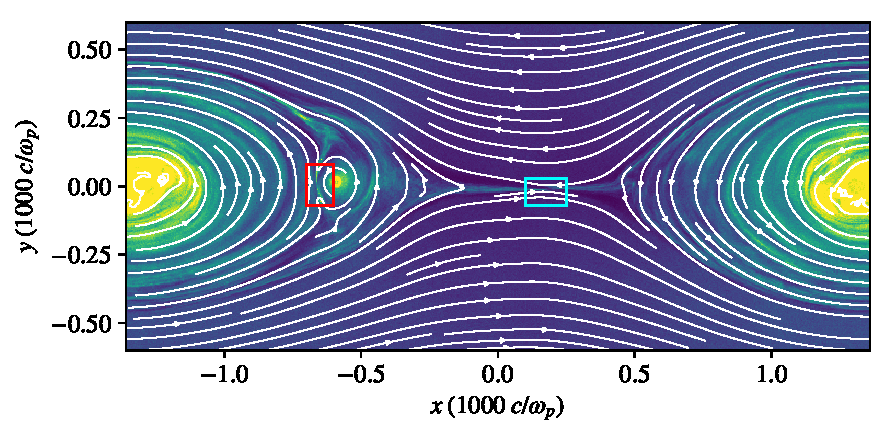
\includegraphics[width=\linewidth]{testing_blines.pdf}
	\caption{Snapshot of density from a triggered simulation with a guide field.  We superimpose streamlines of the in-plane magnetic field and emphasize two regions: the cyan box where reconnection is taking place in the initial horizontal current layer, and the red box, where reconnection is occurring between two merging plasmoids.  Note that the sign of $\vec{\nabla}\times \vec{B}$, and hence the sign of the electric field is positive in the horizontal layer (cyan box), and negative in the vertical current layer between plasmoids (red box).
	}
	\label{blines}
\end{figure*}



To find all the particles at a given time that are accelerated by x-points, we first identify x-points from the fields as described above in \ref{xpoint_id}.  Generally, after a particle is accelerated at an x-point, it either enters a plasmoid or an outflow and moves away from the x-point.  The outflow moves at $\sim v_{A}$, while plasmoids generally move slower than this; the maximum speed that particles move away from x-points is $\sim v_{A}$.  Because of that, we look for all particles that have acceleration episodes that are Alfv\'enically connected to an x-point, i.e., we require that 

\begin{equation}
\lvert\frac{x_{cs} - x_{xpoint}}{t_{cs}-t_{xpoint}}\rvert \le v_{A}.
\end{equation}

In order to identify particle acceleration episodes that are associated with mergers, we exploit the geometry of reconnection at the interface of merging plasmoids.  As mentioned above, in a plasmoid merger, the sign of the electric field will be opposite that in the horizontal current layer's x-points. As such, if the $E_{z}$ field is negative at the time of a particle's acceleration and the particle is Alfv\'enically connected to an x-point, we identify the acceleration episode as being due to an x-point generated in the merger.

If neither of the above criteria are met, we classify the episode as ``other''.  We find that these uncategorized episodes generally produce much lower-energy particles than x-points or mergers, and they are often associated with plasmoid motion, contraction, or the interaction of an outflow with a plasmoid.  

We note that with our classification scheme, while all of the particles accelerated at an x-point will be identified correctly, it will also classify particles that were accelerated near the x-point through other mechanisms.  A particle may be accelerated by some other mechanism near an x-point, but due to our relatively loose criterion (simply Alfv\'enic connection between the acceleration episode and the x-points location), we may classify it as being due to an x-point.  

%\begin{figure}[b]
%	\includegraphics[width=.95\linewidth]{4x1_timespec.png}
%	\caption{Time evolution of the electron energy spectra from our four fiducial simulations, shown in the same order as in Figure \ref{lowbeta_fourdens}.  Time increases from yellow to blue, and the red line depicts the spectra from the final timestep.  We see that the untriggered zero guide field case has the hardest spectra, consistent with the fact that this simulation has the most x-points and plasmoid mergers.
%	}
%	\label{4x1_timespec}
%\end{figure}



\section{Acceleration Results}
In order to assess the relative importance of x-points and plasmoid mergers to the overall electron energy spectra, we iterate through time over all of our simulations and examine the cumulative spectra from the different acceleration mechanisms.  That is, at each output timestep, we identify the location of x-points as described in Section \ref{xpoint_id}.  We then associate all the particles with an acceleration mechanism as described in Section \ref{acc_mec_def}.  We then construct time-integrated energy spectra from these different components and assess their relative importance.
\begin{figure}[htp]
	{
		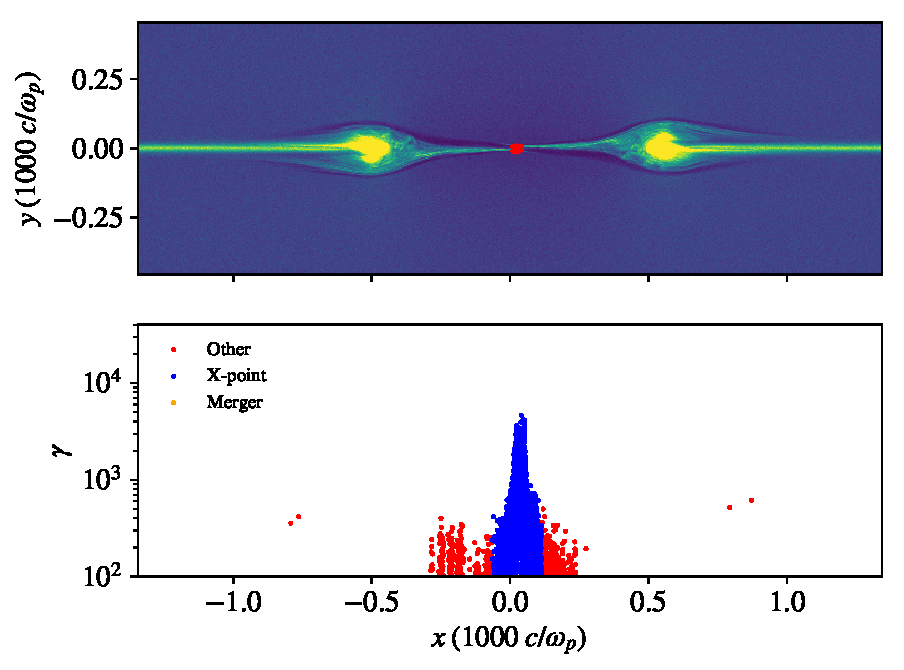
\includegraphics[width=\linewidth]{bguide3_triggered_snap9.pdf}
	}
	\newline
	{
		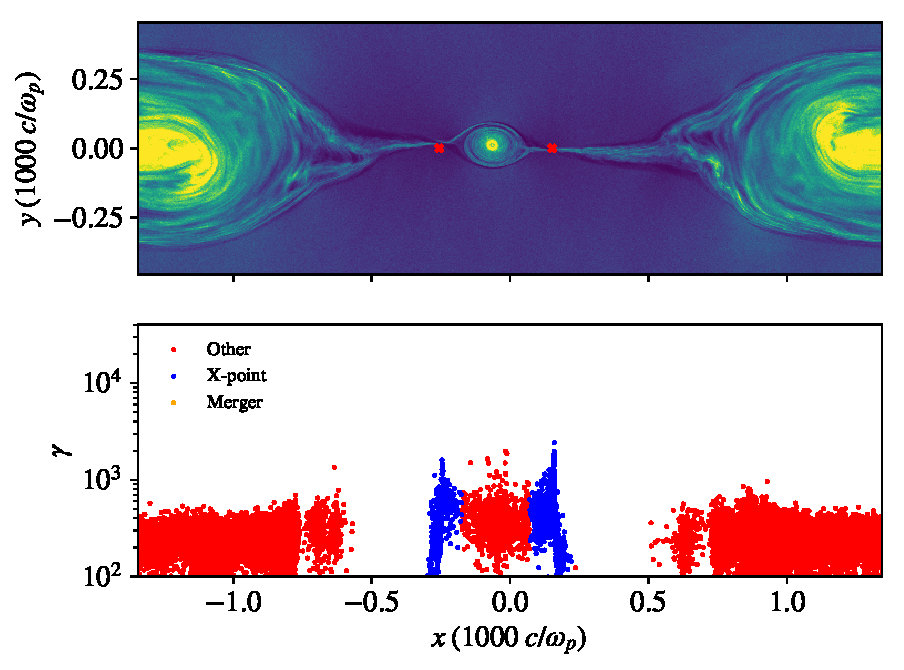
\includegraphics[width=\linewidth]{bguide3_triggered_snap33.pdf}
	}
	\newline
	{
		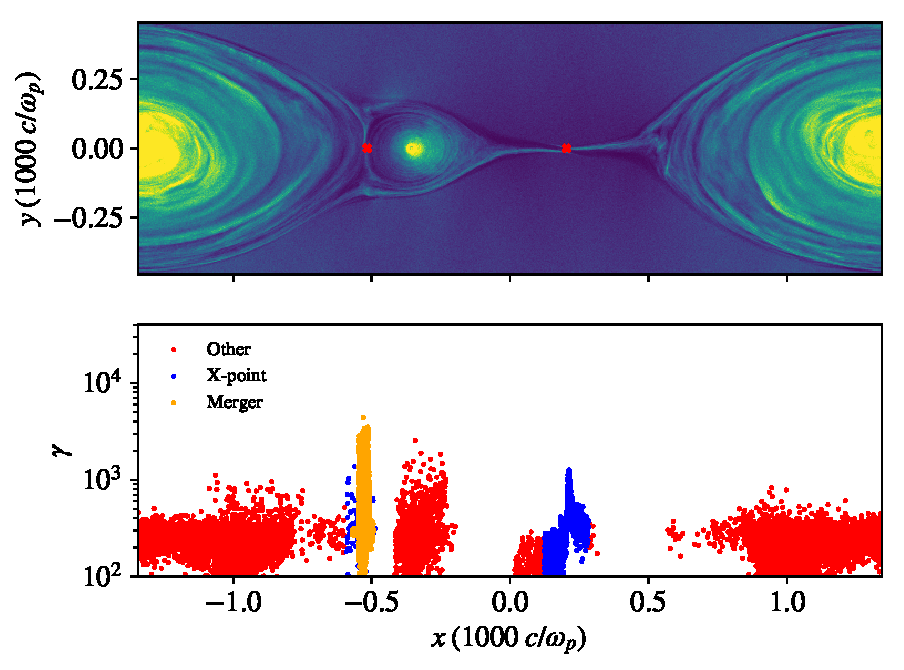
\includegraphics[width=\linewidth]{bguide3_triggered_snap46.pdf}
	}
	
	\caption{Snapshots at three different times from the triggered simulation with a guide field strength of $B_{g}=0.3B_{0}$.  X-points are the dominant sites of electron acceleration and there are very few of them throughout the simulation.  One secondary plasmoid forms (middle two panels), and eventually merges into the boundary island (bottom two panels), which also accelerates some particles.
	}
	\label{triggered_bguide_snapshots}
\end{figure}


\begin{figure}[htp]
	
	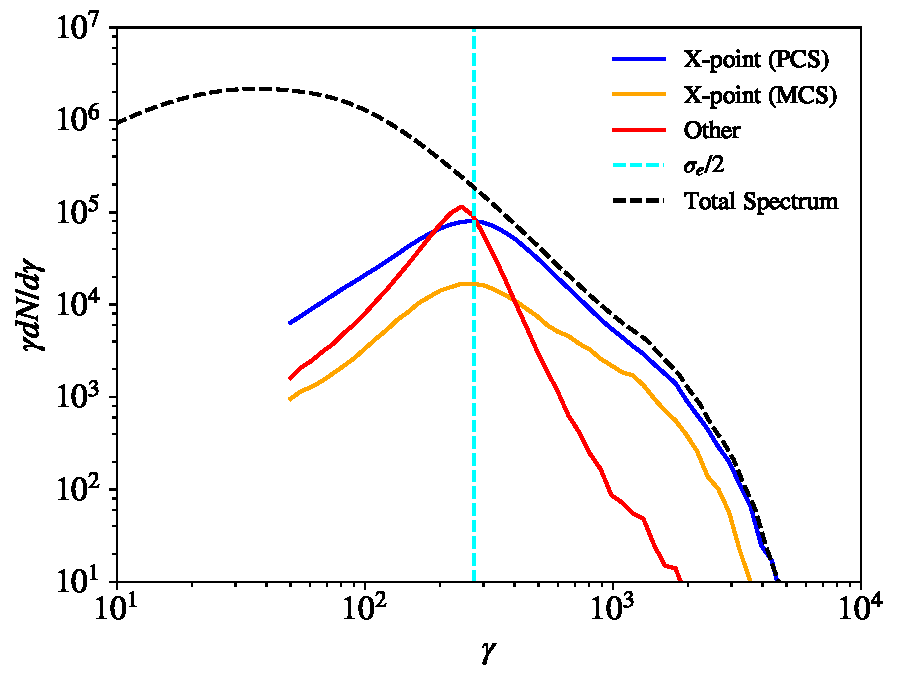
\includegraphics[width=\linewidth]{bguide3_triggered_withspec.pdf}
	\caption{Time-integrated electron spectra from the triggered simulation with guide field $B_{g}=0.3B_{0}$ decomposed by acceleration mechanism.  X-points dominate the majority of the high-energy electron acceleration, with a modest contribution from the single merger that happens during this simulation.}
	\label{triggered_bguide_spec}
\end{figure}


We show in Figure \ref{triggered_bguide_snapshots} three snapshots in time from the triggered simulation with a guide field strength of $B_{g}=0.3B_{0}$, which suppresses the secondary tearing mode.  Each timestep is depicted with two panels: the top panel shows the density profile, and the bottom panel depicts the location where the particle first exceeds $\sigma_{e}/2$ versus the particle's final energy. 

We see that at an early time (top two panels), there is a single primary x-point accelerating particles to high energies.  As reconnection proceeds, a single secondary plasmoid begins to develop in the middle of the domain (middle two panels), and there are two corresponding secondary x-points on either side.  These secondary x-points accelerate particles, but not as prolifically as the initial primary x-point.  Eventually, the plasmoid is pulled towards the left edge of the domain (bottom two panels) and merges with the large boundary island.  A current sheet forms between the two plasmoids and their magnetic fields reconnect, serving as another site of acceleration, with the expected flip in $E_{z}$ polarity from the x-points in the initial current sheet.  

We show the time-integrated spectra from the different mechanisms in Figure \ref{triggered_bguide_spec}.  In this case, the majority of the high-energy particles ($\gamma \geq 300$) come from x-points, and in particular, the primary x-point.  This is because the guide field suppresses secondary x-point and plasmoid formation, resulting in only one merging event over the course of the simulation.  We note that because acceleration is so localized in this case, in the limit of very large domains, the acceleration region will comprise a vanishing fraction of the total domain and we expect acceleration to be negligible.  

%\begin{figure}[!h]
%	{
%		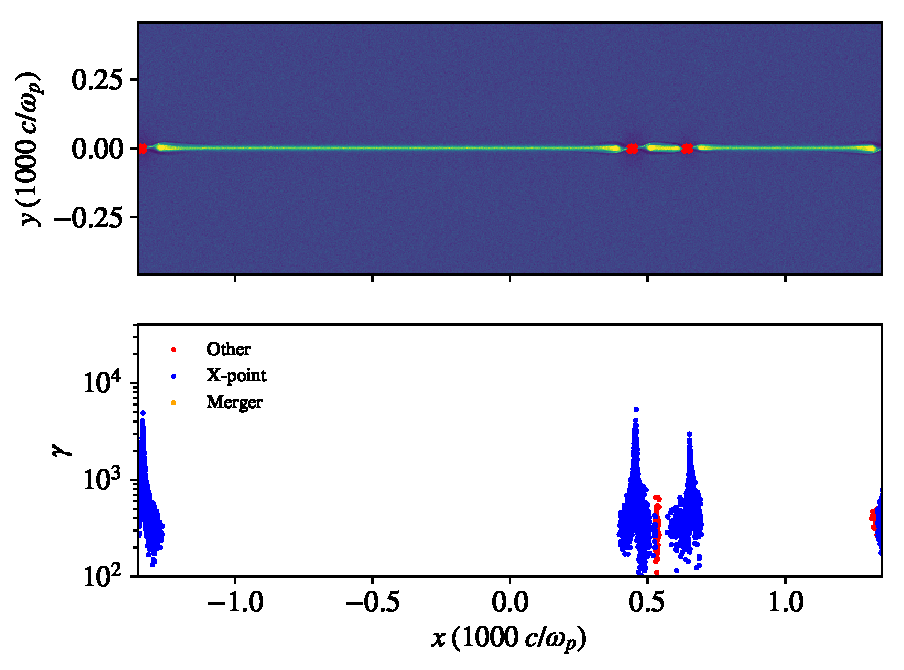
\includegraphics[width=\linewidth]{bguide3_untriggered_snap6.pdf}
%	}
%	\newline
%	{
%		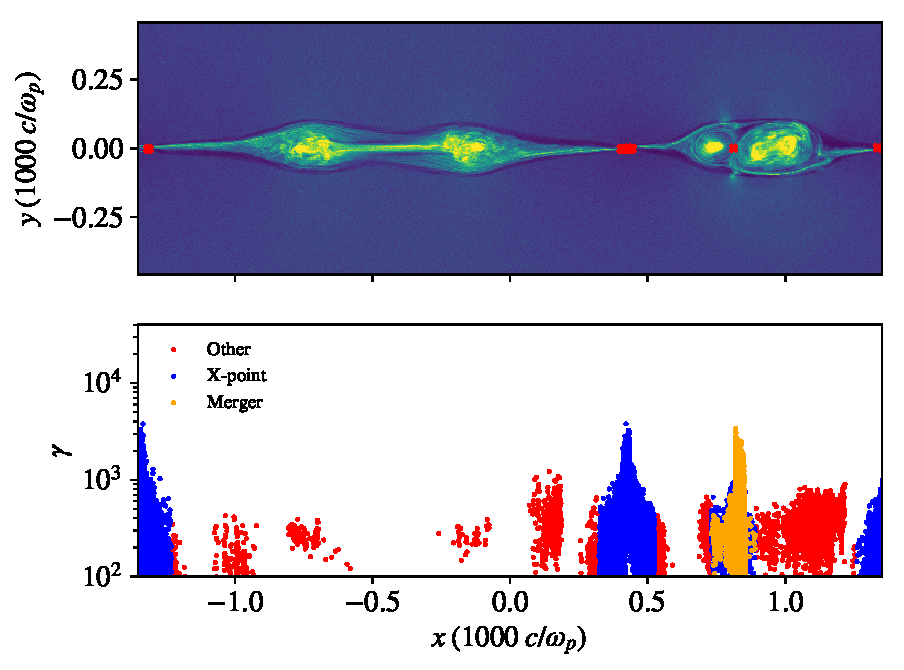
\includegraphics[width=\linewidth]{bguide3_untriggered_snap12.pdf}
%	}
%	\newline
%	{
%		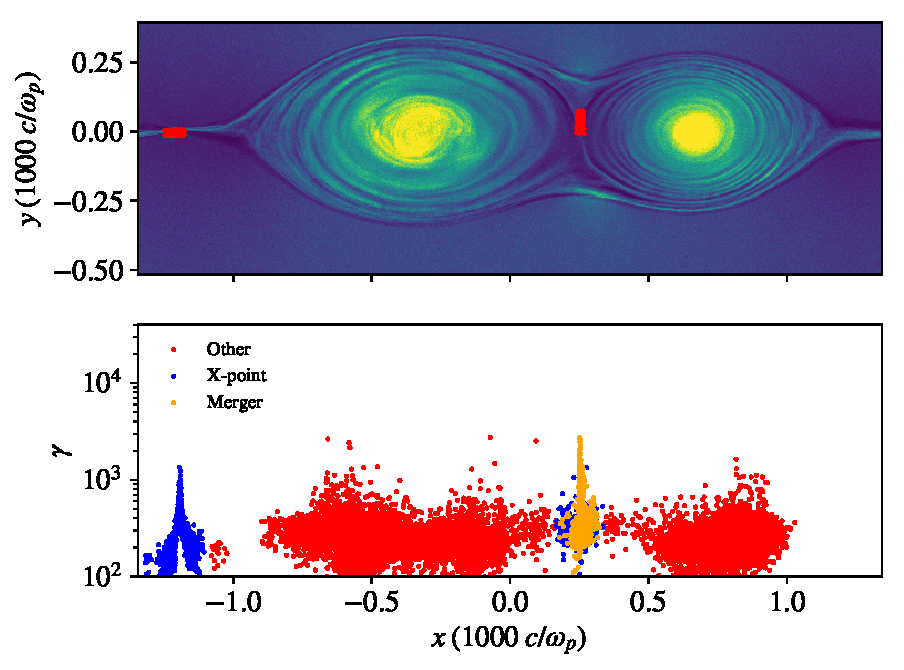
\includegraphics[width=\linewidth]{bguide3_untriggered_snap44.pdf}
%	}
	
%	\caption{Snapshots at three different times from the untriggered simulation with a guide field strength of $B_{g}=0.3B_{0}$.  Because we do not trigger reconnection, numerous primary x-points form and we see numerous primary x-points and plasmoid mergers throughout the simulation domain.
%	}
%	\label{untriggered_bguide_snapshots}
%\end{figure}

%In order to explore the effect of having numerous primary x-points, we show in Figure \ref{untriggered_bguide_snapshots} snapshots from the untriggered simulation with the same guide field strength of $B_{g}=0.3B_{0}$.  At early times (top two panels), we see the primary tearing mode pinch the current sheet at three locations, resulting in three primary x-points, all of which serve as sites of particle acceleration.  In the middle two panels, we see two of the primary plasmoids merging at $x \approx 0.77$, accelerating numerous particles.  In an untriggered setup, such as this one, the primary plasmoids hierarchically merge, resulting in very large plasmoid mergers at late times, which we see in the bottom panels.  As these large plasmoids merge, they accelerate a large number of particles as their magnetic fields reconnect.  

%We show the cumulative spectra from this simulation in Figure \ref{untriggered_bguide_spec}.  We see that x-points are still the dominant source of high-energy particles.  In fact, the slope of the x-point is even harder than in the triggered case: there are many more high-energy particles in the untriggered simulation.  This is because whereas in the triggered setup there is only one relevant x-point in the system, and it takes up a fairly small fraction of the length of the current sheet.  In the untriggered setup, however, there are three times as many primary x-points, which means more particles interact with an x-point and are able to be accelerated to highly relativistic energies.  In this simulation, mergers are still subdominant to x-points in their contribution to producing high-energy electrons.  We note that the contributions to high-energy particle acceleration between x-points and mergers is likely a function of the number of x-points per unit length in the sheet.  As such, the initial thickness of the current sheet in an untriggered setup plays an important role in setting the relative importance of x-points and mergers, and will affect the the overall spectrum of non-thermal particles.  


%\begin{figure}[htp]
%	{
%		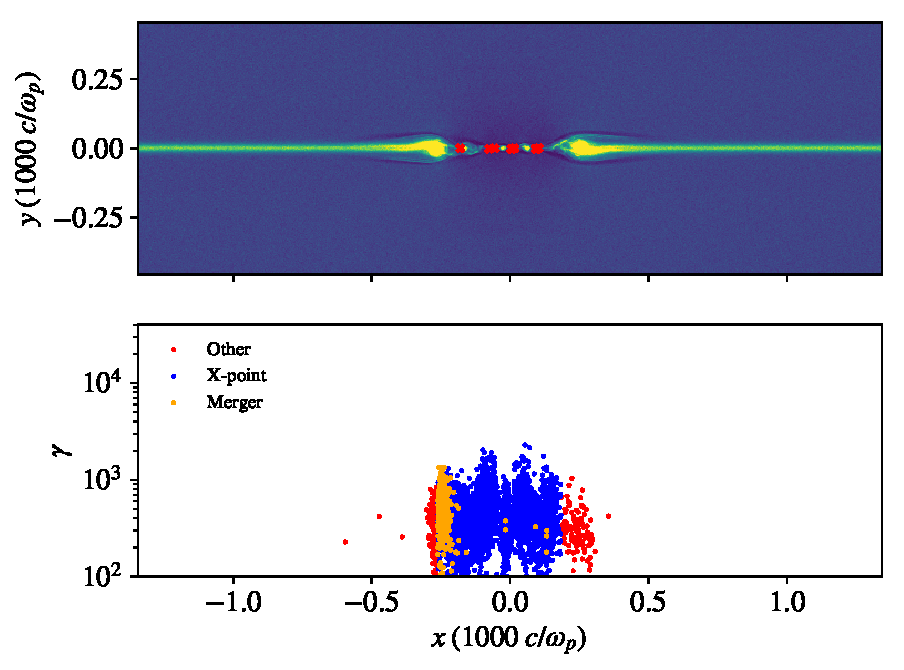
\includegraphics[width=\linewidth]{bguide1_triggered_snap6.pdf}
%	}
%	\newline
%	{
%		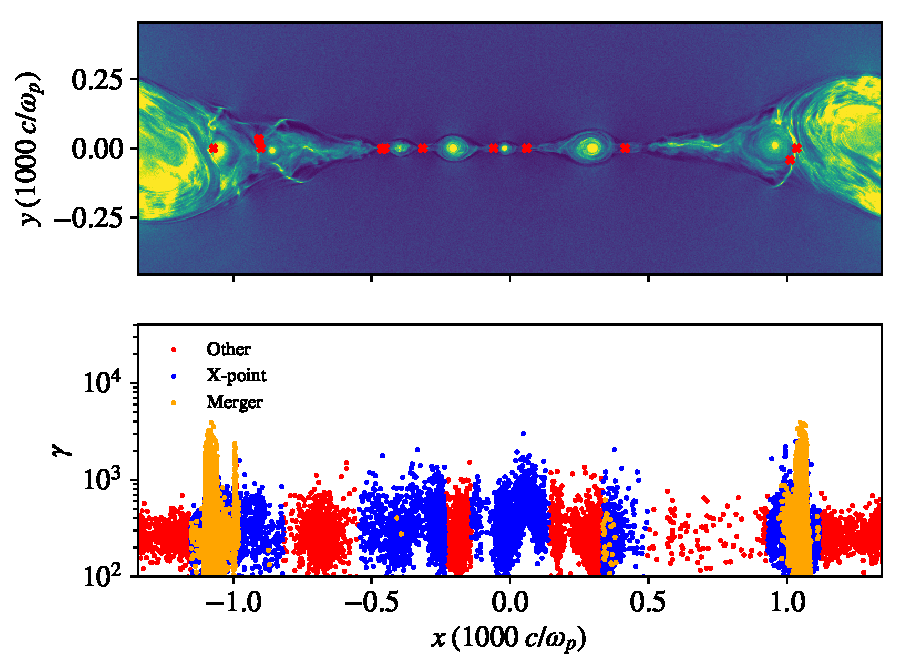
\includegraphics[width=\linewidth]{bguide1_triggered_snap020.pdf}
%	\newline
%	{
%		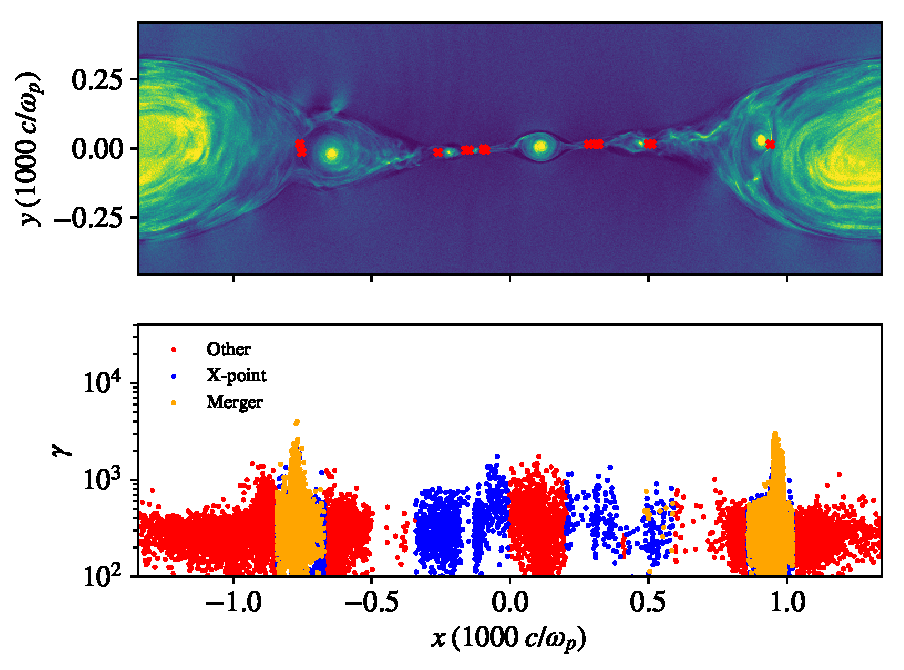
\includegraphics[width=\linewidth]{bguide1_triggered_snap28.pdf}
%	}
%	
%	\caption{Snapshots at three different times from the triggered simulation with $B_{g}=0.1B_{0}$.  The secondary tearing mode fractures the current sheet throughout the domain, resulting in numerous x-points and secondary plasmoids.  
%	}
%	\label{triggered_bguide0_snapshots}
%\end{figure}

%We show in Figure \ref{triggered_bguide0_snapshots} three snapshots from the triggered simulation with no guide field.  We see at early times that numerous closely-spaced secondary x-points have already formed in the region vacated by the reconnection fronts.  Two small plasmoids at $x\approx 0.1$ are merging.  Due to the prevalence of the secondary tearing mode and associated plasmoid mergers, acceleration is not as localized as in the previous cases with a guide field.  This trend continues in the middle panel, where secondary x-points are accelerating particles all throughout the central $\sim 1/3$ of the domain.  The secondary plasmoids that form are inevitably pulled towards the edge of the domain, ultimately merging with the large boundary island, accelerating particles in merging events.  This trend continues to later times (bottom panels): acceleration at secondary x-points and the associated merging of secondary plasmoids remains active until the magnetic island at the boundary grows so large that it chokes off the inflowing plasma and reconnection halts.  

%When we compare the relative contributions of x-points and mergers to the electron energy spectrum, in Figure \ref{triggered_bguide0_spec}, we find that both x-points and mergers accelerate a large number of particles above $\gamma=1000$.  Mergers slightly dominate over x-points in overall number of particles that are accelerated to these highly relativistic energies.

In Figure \ref{untriggered_bguide0_snapshots} we show three snapshots from the untriggered simulation with $B_{g}=0.1B_{0}$.  This is the simulation with most x-points and plasmoids due to the fact that the secondary tearing mode is active, as well as it being an untriggered simulation.  This guarantees that there will be numerous mergers of varying sizes, from small secondary plasmoids merging with one another, to the larger primary plasmoids hierarchically merging until the system on consists of one large plasmoid.  At early times (top panel), numerous primary and x-points quickly form and begin accelerating at these specific locations.  We see that 4 primary plasmoids form out of the 4 initial x-points that spontaneously develop and segment the current layer at $x\approx -1.5, \; -0.75, \; -0.4, \;$ and $0.3$.  In the middle two panels, we see the four large primary plasmoids, two of which are beginning to merge at $x \approxeq -0.4$.  In addition to these primary plasmoids merging, we see the formation and subsequent merging of secondary plasmoids throughout the reconnection layer.  We see that the x-points that occur frequently in the layer continue to accelerate particles, while the plasmoid mergers also contribute considerably.  In this case, because mergers and x-points are so prevalent throughout the simulation, a particle's final energy is not as critically dependent on its first interaction with the current sheet being at an x-point: when the secondary tearing mode is active, acceleration occurs throughout the domain due to the prevalence of x-points and plasmoid mergers. 

We show in Figure \ref{untriggered_bguide1_spec} the spectra of particles from the simulation shown in Figure \ref{untriggered_bguide0_snapshots}.  We see that due to the large number of plasmoid mergers that occur all throughout the domain, that the majority of the high-energy electrons are energized in merging events.  X-points still play a considerable role, but are not dominant like they were in the case where the secondary tearing mode was suppressed.  Interestingly, the acceleration episodes categorized as ``other'' are much more significant in this case than in the previous case we considered.  This is likely because of the turbulent motions induced by plasmoid mergers, as well as the fact that electrons in this simulation are much more likely to experience multiple stages of acceleration due to the large number of plasmoids in the system.  For example, if a particle enters a plasmoid and eventually exceeds the energy threshold due to the contraction of the plasmoid, it will be categorized as ``other''.  However this plasmoid will eventually merge with another and may further energize the particle.  Because of this, we expect that in systems with many mergers that particles classified as ``other'' should have higher energies than a system with very few or no mergers, such as in the triggered case with $B_{g}=0.3B_{0}$.  Indeed this is reflected in a comparison of the spectra: the ``other'' component is significantly harder and extends to higher energies in the case with more mergers.



\begin{figure}[!h]
	{
		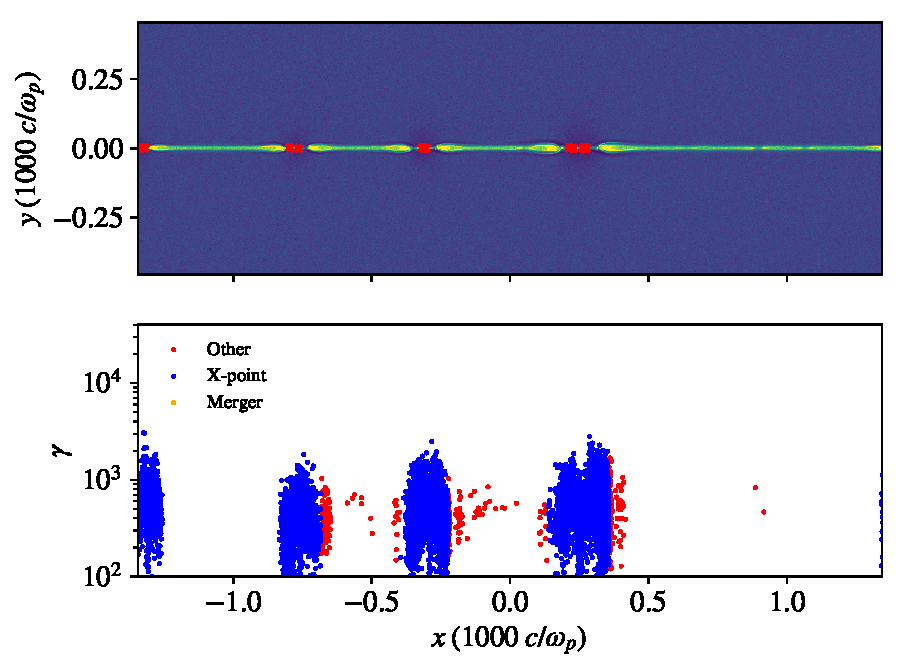
\includegraphics[width=\linewidth]{bguide1_untriggered_snap7.pdf}
	}
	\newline
	{
		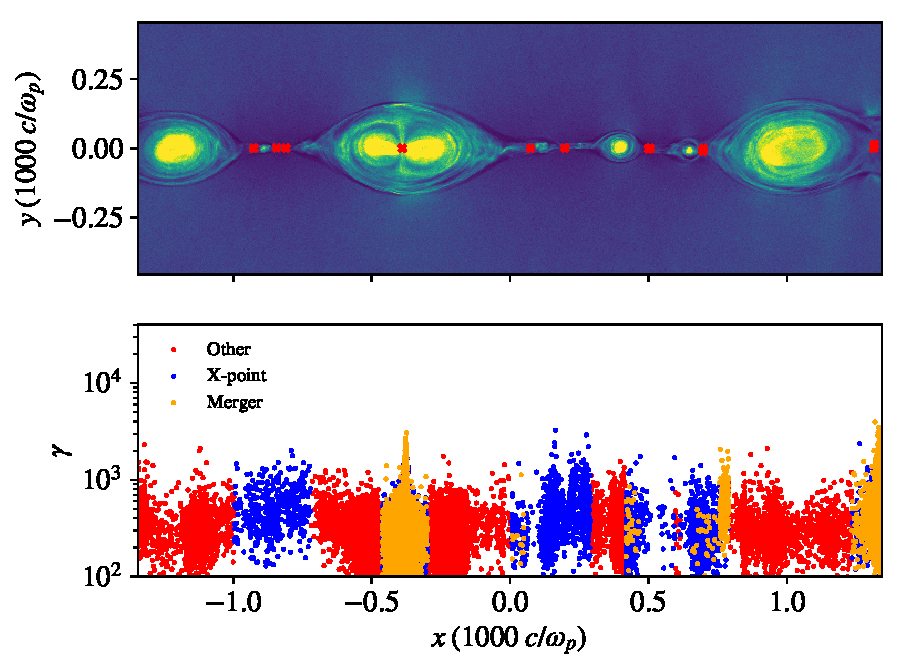
\includegraphics[width=\linewidth]{bguide1_untriggered_snap20.pdf}
	}
	\newline
	{
		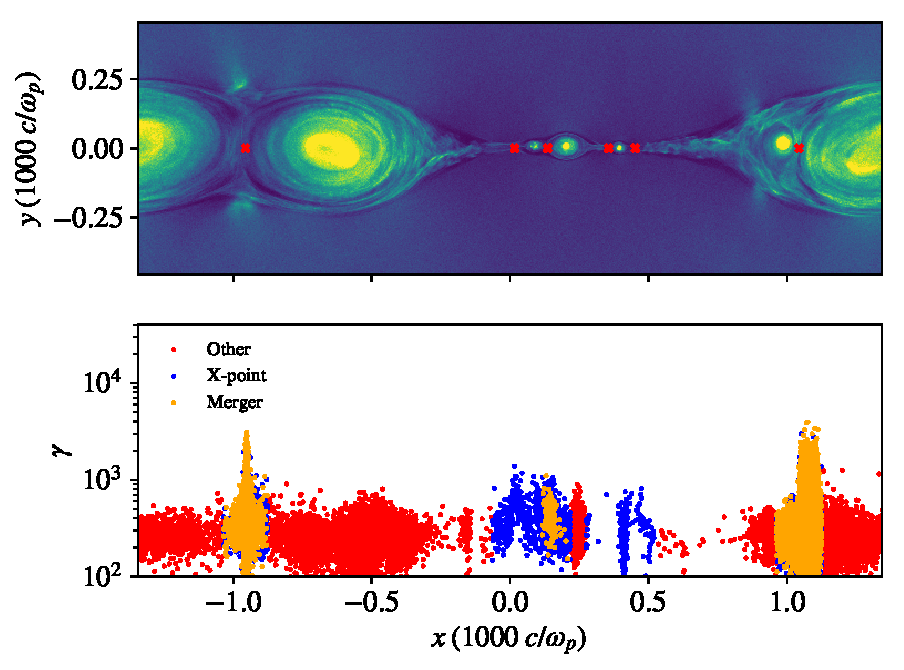
\includegraphics[width=\linewidth]{bguide1_untriggered_snap30.pdf}
	}
	
	\caption{Snapshots at three different times from the untriggered simulation with no guide field.  We see that both the primary and secondary tearing mode result in copious x-point and plasmoid formation and the corresponding electron acceleration.  
	}
	\label{untriggered_bguide0_snapshots}
\end{figure}

\begin{figure}[htp]
	
	\includegraphics[width=\linewidth]{bguide1_untriggered_withspec.pdf}
	\caption{Time-integrated electron spectra from the untriggered simulation with no guide field.  The prevalence of plasmoids (both primary and secondary), and their merging results in plasmoid mergers dominating over x-points for high-energy acceleration.}
	\label{untriggered_bguide1_spec}
\end{figure}


We show in Figure \ref{untriggered_bguide3_spec} the spectra decomposed by acceleration mechanisms from our untriggered $B_{g}=0.3B_{0}$ simulation.  A snapshot of the density structure of this simulation can be seen for reference in the lower right panel of Figure \ref{lowbeta_fourdens}.  In Figure \ref{untriggered_bguide3_spec}, we see that x-points continue to dominate the production of high-energy electrons, as in the triggered case with the same guide field strength (Figure \ref{triggered_bguide_spec}).  We see that x-point acceleration is naturally enhanced in the untriggered setup because there are (in this case) three primary x-points as compared to the single primary x-point in the triggered setup.  Interestingly, however, the relative contribution to the overall spectrum from mergers as compared to x-points is slightly less significant in the untriggered setup.   We can explain this initially puzzling result by comparing the ratio of primary x-points to mergers in each simulation.  In our triggered $B_{g}=0.3B_{0}$ simulation, there is one primary x-point and one plasmoid merger, so $N_{\rm{x}}/N_{\rm{merge}}=1$.  In an untriggered setup where no secondary plasmoids form, the number of mergers is always $N_{\rm{merge}}=N_{\rm{x}}-1$.  In our particular case, there are three primary x-points, which means that $N_{\rm{x}}/N_{\rm{merge}}=3/2$.  Following this logic, we would expect the ratio of x-point to merger accelerated particles in the triggered case to be $2/3$ of that for the untriggered case.  We now test whether or not this hypothesis could plausibly explain the difference between these triggered and untriggered simulations.  First we calculate the ratio of the number of particles accelerated by an x-point versus a merger at a representative Lorentz factor, $\gamma = 1000$.  We call this ratio $$R \equiv \frac{dN_{\rm{xpoint}}/d\gamma}{dN_{\rm{merge}}/d\gamma}|_{\gamma=1000}.$$  We calculate this ratio for both our triggered and untriggered case, yielding values of $R_{\rm{triggered}}=2.5$ and $R_{\rm{untriggered}}=3.5$.  The ratio of these values, $R_{\rm{triggered}}/R_{\rm{untriggered}}=0.71$ is indeed close to $2/3$, showing that the relative number of primary x-points to plasmoid mergers may explain the differences we see between the x-point and merger's contributions to the production of high-energy particles between our untriggered and triggered setup with $B_{g}=0.3B_{0}$, where secondary plasmoid formation is suppressed.

\begin{figure}[htp]
	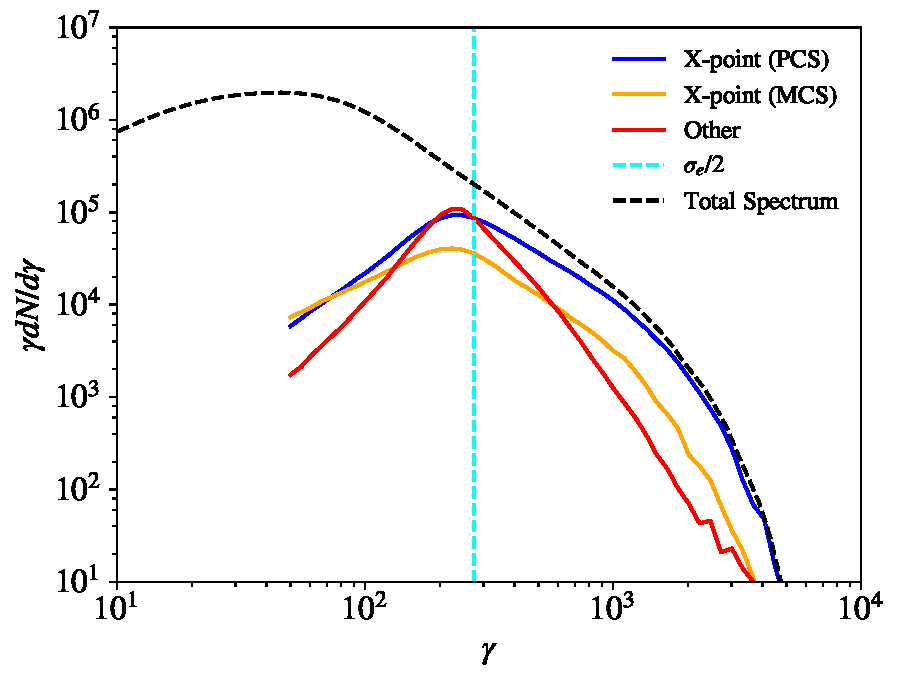
\includegraphics[width=\linewidth]{bguide3_untriggered_withspec.pdf}
	\caption{Time-integrated electron spectra from the untriggered simulation with $B_{g}=0.3B_{0}$.  We see that x-point acceleration continues to dominate the cumulative high-energy spectrum of electrons. }
	\label{untriggered_bguide3_spec}
\end{figure}

We show in Figure \ref{triggered_bguide1_spec} the spectra decomposed by acceleration mechanisms from our triggered $B_{g}=0.1B_{0}$ simulation.  A snapshot of the density structure of this simulation can be seen for reference in the upper left panel of Figure \ref{lowbeta_fourdens}.  We see that due to onset of the secondary tearing mode, that mergers dominate the overall spectrum, as in the untriggered case in Figure \ref{untriggered_bguide1_spec}, with a similar overall shape of the merger spectrum, but with a lower normalization because there will naturally be more mergers in an untriggered setup.  Additionally, we see that the x-point spectrum is slightly less significant in the triggered setup, which also occurs simply because  untriggered setups have numerous primary x-points as compared to the single primary x-point of a triggered setup.



\begin{figure}[htp]
	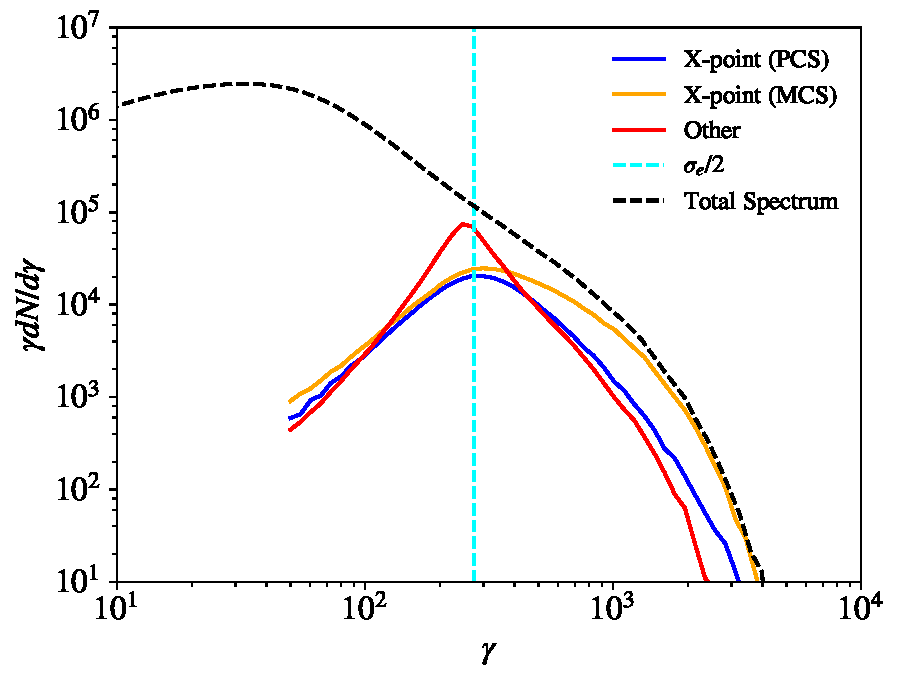
\includegraphics[width=\linewidth]{bguide1_triggered_withspec.pdf}
	\caption{Time-integrated electron spectra from the triggered simulation with $B_{g}=0.1B_{0}$.  Even when reconnection is triggered, the onset of the secondary tearing mode produces numerous secondary plasmoids, leading to a merger-dominated spectrum.}
	\label{triggered_bguide1_spec}
\end{figure}


\section{Investigating the non-ideal Electric Fields}\label{E_comps}
In the previous sections we explored where electrons are first accelerated and found that x-points appear to be important structures in regulating the production of a non-thermal electron spectrum.  In this section, we explore in more detail the energetics and dynamics of electrons that are accelerated by the non-ideal electric fields near an x-point. 

As previously discussed, x-points have a strong non-ideal out-of-plane (in the $\pm \hat{z}$ direction) electric field associated with them.  This electric field is aligned with the guide field and results in a large $|\vec{E}\cdot\hat{b}|$ with the dominant component being from the z-aligned electric field near the x-point.  We show the structure of $E_{||}$ and its various components from our triggered simulation with $B_{g}=0.3B_{0}$ in Figure \ref{edotb_comps}.  We see that the parallel electric field near the x-point is dominated by the z-component of the electric field, as expected.  In the outflows, however, there is a significant component of $E_{||}$ in the x-direction (along the outflow).  Ultimately we will see that when particles interact with the z-aligned electric field near the x-point, that they are likely to be accelerated beyond the thermal peak of the spectrum into a non-thermal tail, whereas particles that interact with $E_{||}$ along the outflow make up the thermal peak of the distribution.  
\begin{figure*}[htp] 
	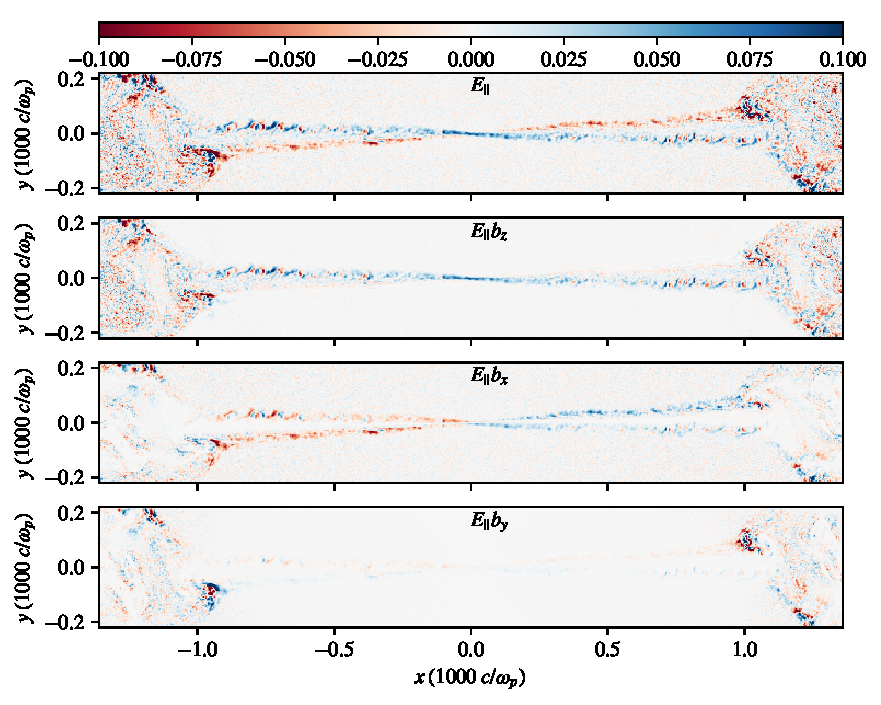
\includegraphics[width=\linewidth]{testing_singleplot_flds.pdf}
	\caption{Profiles of the parallel electric field (top), decomposed into its Cartesian components (bottom three) for a high-energy electron from the triggered simulation with $B_{g}=0.3B_{0}$.  We see that the parallel electric field near the x-point is dominated by the z-component associated with the dissipation at the x-point.  A significant parallel electric field persists in the edges of the outflow, largely from the x-component of $E_{||}$.  The y-component is negligable except in small localized regions where the dense parts of the outflow are impacting the magnetic island, generating turbulent motions in the large boundary island (i.e., at $x\approx \pm 1$, $y\approx \pm 1$ in the bottom panel). }
	\label{edotb_comps}
	\end{figure*}

In order to statistically assess the importance of electron energization by $E_{||,z}$ at x-points, we track in our simulation the total work done on each particle by the parallel component of the electric field in the z-direction, $$W_{||,z}=\int_{t_{0}}^{t_{f}}{qE_{||}b_{z}}v_{z}dt$$ where $E_{||}=\vec{E}\cdot\hat{b}$, $b_{z}$ is the z-component of the unit vector pointing in the direction of the local magnetic field, and $v_{z}$ is the z-velocity of the particle.  We show in Figure \ref{wpar_hist_earlytime} a 2d histogram of the z-component of parallel work versus Lorentz factor from our triggered simulation with $B_{g}=0.3B_{0}$ at both an early time before the formation of any magnetic islands (top) and a later time (bottom) when the boundary island has formed and a single plasmoid has formed and merged into it (see Figure \ref{triggered_bguide_snapshots}).  At early times, we see that the parallel electric field in the z-direction at the primary x-point is responsible for all particles above $\gamma \sim 200$.  At later times, we see that processes not associated with $W_{||,z}$ have resulted in the energization of a large number of electrons.  We can see this because the dispersion away from the $\gamma=W_{||,a}$ line is much greater at later times.  This happens because at early times, there are not many processes operating that will energize electrons: the only available mechanisms are at the x-point, or being swept up in the outflow.  At later times, however, the physics become more complicated.  Electrons can be energized through the interaction of the outflow with the magnetic island, in the turbulence generated when the reconnection fronts interact across the boundary, in the vicinity of a plasmoid merger, or in a contracting magnetic island.  


\begin{figure}[htp] 
	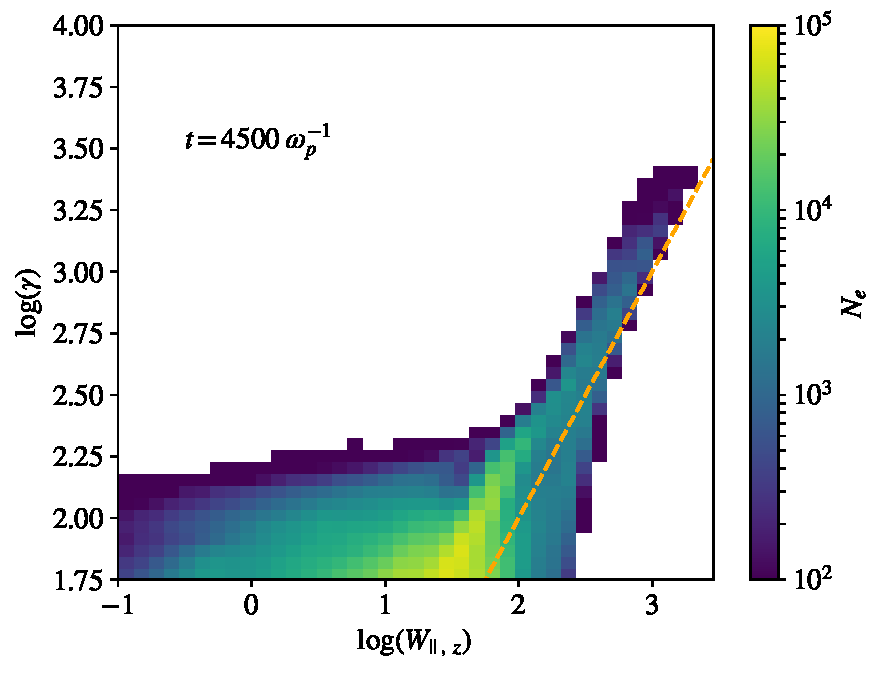
\includegraphics[width=\linewidth]{bguide3_triggered_final_wparz_gam_t15.pdf}
	\newline
	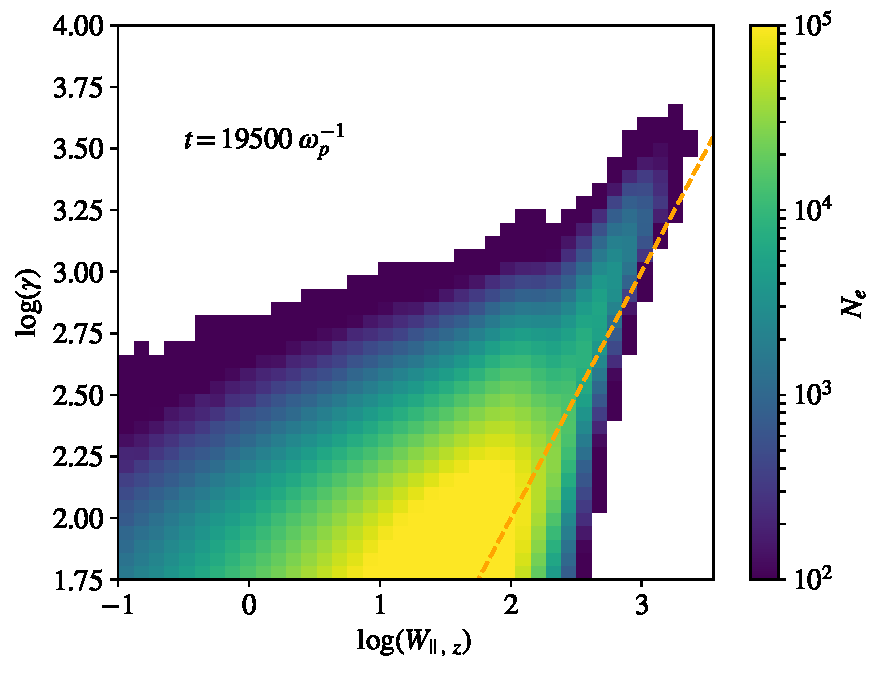
\includegraphics[width=\linewidth]{bguide3_triggered_final_wparz_gam_t65.pdf}
	
	\caption{2d histograms of the z-component of parallel electric field work versus Lorentz factor taken at two different times from the triggered $B_{g}=0.3B_{0}$ simulation.  The dashed orange line depicts $\gamma = W_{||,z}$.  The top panel corresponds to a relatively early time in the simulations when the reconnection fronts have not interacted across the boundary.  The bottom panel corresponds to a later time when the large magnetic island at the boundary has formed. }
	\label{wpar_hist_earlytime}
\end{figure}


In order to give some examples of individual particles, we show the evolution of a few representative electrons' Lorentz factor as well as the work done by the z-component of the parallel electric field from the triggered simulation with $B_{g}=0.3B_{0}$ in Figure \ref{EdotV}.  Each color refers to an individual particle, with the solid line corresponding the particle's Lorentz factor, and the dashed line representing $W_{||,z}$.  The highest-energy particle (blue line) is typical of the highest energy electrons in the system: it is first energized in an interaction with the primary x-point, where it is rapidly accelerated to $\gamma \sim 1000$ by $E_{||,z}$.  After this, it gains a bit more energy as it bounces around in the contracting magnetic island through processes not associated with $E_{||,z}$.  The orange particle's trajectory is slightly different: it is first energized to $\gamma \sim 200$ when it interacts with the outflow, which is driven largely by $E_{||,x}$, so $W_{||,z}$ does not follow the particle's energization at this step.  It enters the large boundary magnetic island, where its energy oscillates until the secondary plasmoid merges into the boundary island, at which point this particle interacts with the current sheet in between the two merging plasmoid and experiences a large $E_{||,z}$, increasing the work done by this non-ideal electric field, and further accelerating the particle to higher energies.  The green particle, in contrast, never experiences a particularly strong $E_{||,z}$, and hence its energy remains in the thermal peak of the spectrum.  The green particle is energized in the same merging event as the particle represented with an orange line, but this particle does not interact with an x-point (and hence $E_{||,z}$) in the current sheet between the two merging plasmoids, but rather gains energy through other means during the merger, and hence does not gain as much energy as the particle that interacts with the strong non-ideal $E_{||,z}$ in the current sheet.

\begin{figure}[htp]
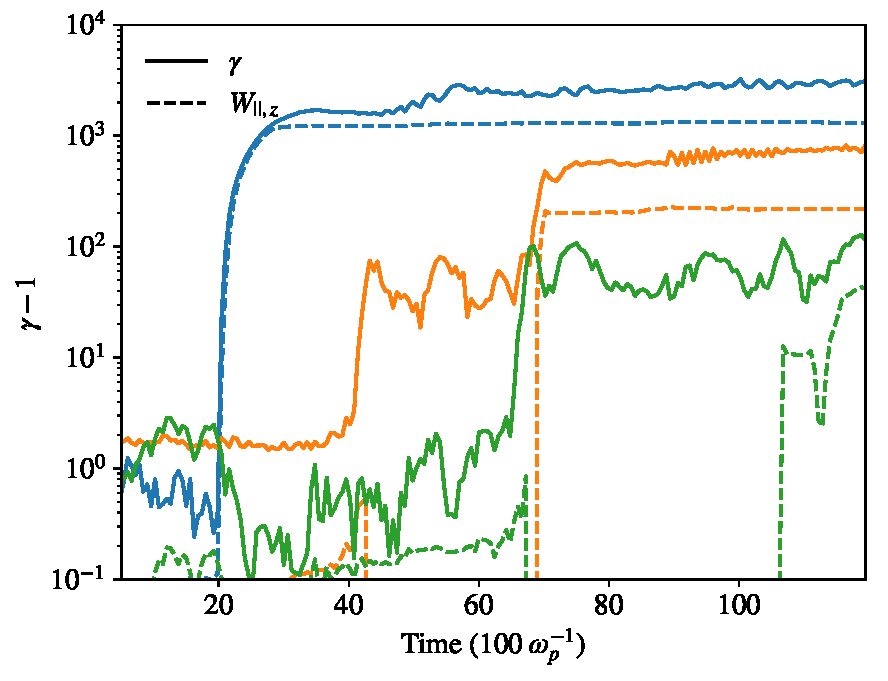
\includegraphics[width=\linewidth]{manypart_wparz_handselect2_lessprt.pdf}
\caption{Evolution of Lorentz factor and the z-component of parallel work, $W_{||,z}$, of a collection of electrons from the triggered simulation with $B_{g}=0.3B_{0}$.  The solid lines represent the electron's Lorentz factor and the dashed lines depict $W_{||,z}$.  }
\label{EdotV}
\end{figure}

We show in Figure \ref{bguide1_wpar_hist} the same 2d histograms for the triggered simulation with $B_{g}=0.1 B_{0}$.  We see in this case that there is still a strong correlation between particle final energy and the work done by the z-component of parallel electric fields: the non-ideal electric field at x-points is still playing an important role in accelerating a large number of non-thermal particles.  However, we see that there is significantly more dispersion away from the $\gamma = W_{||,z}$ than Figure \ref{wpar_hist_earlytime}, where the secondary tearing mode is suppressed.  This is because in an environment with an abundance of secondary plasmoids and x-points, there are more available channels for energy gain that are not necessarily associated with $E_{||,z}$.  

\begin{figure}[htp] 
	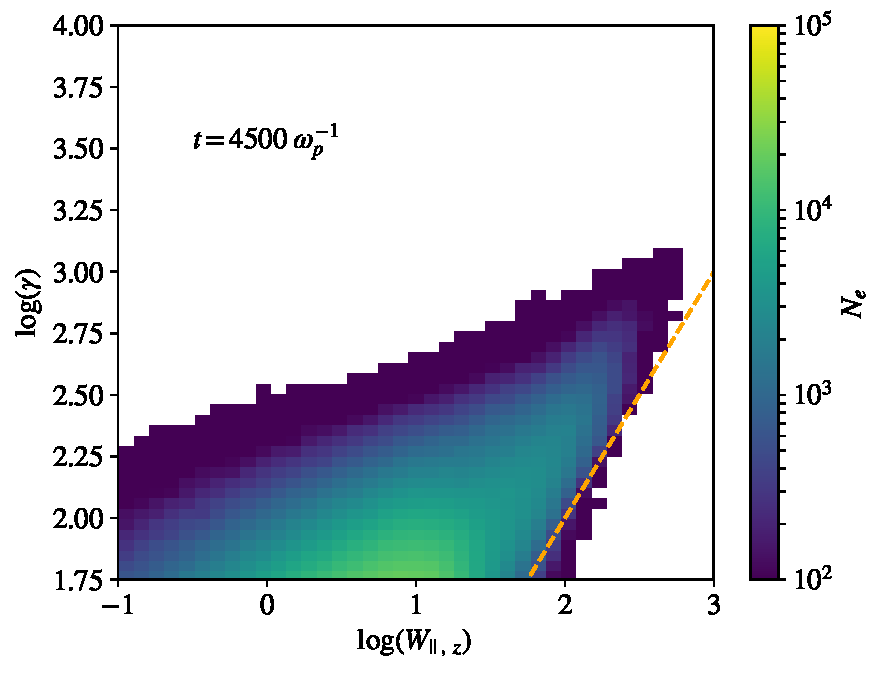
\includegraphics[width=\linewidth]{bguide1_triggered_final_wparz_gam_t15.pdf}
	\newline
	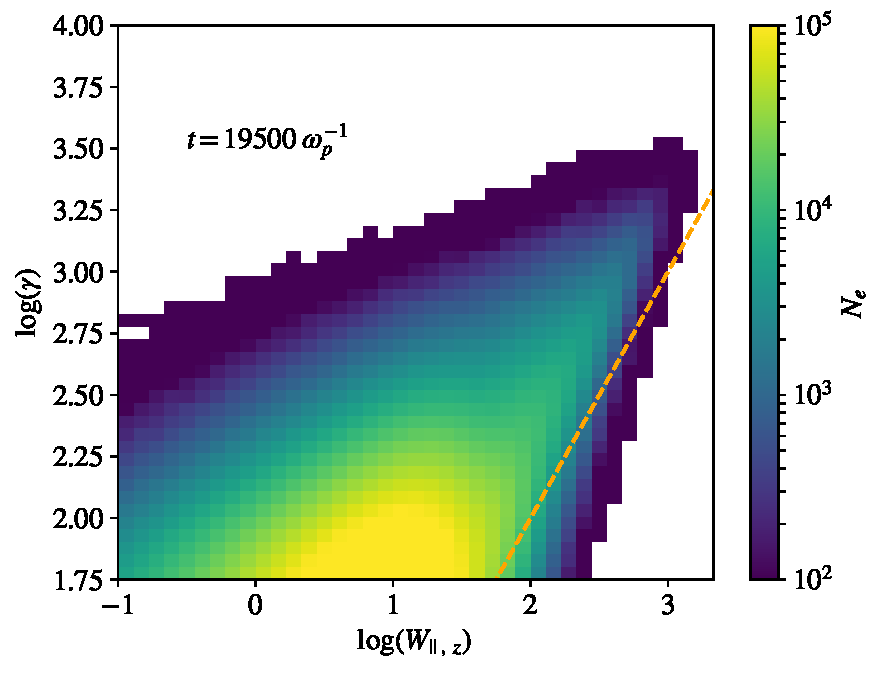
\includegraphics[width=\linewidth]{bguide1_triggered_final_wparz_gam_t65.pdf}
	
	\caption{2d histograms of the z-component of parallel electric field work versus Lorentz factor taken at two different times from the triggered $B_{g}=0.1B_{0}$ simulation.}
	\label{bguide1_wpar_hist}
\end{figure}


\section{The effect of parallel electric fields}\label{test_prtls}
In order to more thoroughly test our finding that non-thermal acceleration is largely controlled by  $E_{||,z}$ at x-points, we include populations of test particles that only feel certain components of $\vec{E}_{||}$.  These particles are evolved simultaneously to the normal particles but do not deposit their currents onto the grid.  We use two sets of test particles to explore the energization mechanism of electrons.  One set of test particles does not feel any electric fields parallel to magnetic fields (i.e., $W_{||}=0$), and the other set does not feel any z-component (out-of-plane) of the $E_{||}$ field ($W_{||,z}=0$).  

We show the spectra of these different populations of particles in Figure \ref{testprtl_spec} for the triggered simulation with $B_{g}=0.3B_{g}$.
We see that the particles that do not experience any $E_{||}$ (red dotted line) are only slightly heated beyond their initial thermal distribution.  This demonstrates that both bulk heating and non-thermal acceleration are mediated by parallel electric fields.  The particles that don't experience $E_{||,z}$, however, have a thermal peak that is consistent with the normal particles at $\gamma \approx 100$, but shows no evidence of a non-thermal distribution above this thermal peak.  This confirms our hypothesis that the non-thermal tail of the distribution is controlled by the parallel electric field in the z-direction associated with the x-point.  The thermal peak is still able to form because particles that enter the current layer in the outflow primarily interact with the outflow-aligned electric field, $E_{||,x}$.

In Figure \ref{bguide1_testprtl_spec}, we show the spectra of test particles for the triggered $B_{g} = 0.1 B_{0}$ simulation.  We see that the test particles that do not experience any parallel electric fields, depicted with the dotted red line, is much more significant than in Figure \ref{bguide1_testprtl_spec}.  This is because in an environment where the secondary tearing mode is active, plasmoids continually form and merge together, providing more sites where plasma motions, plasmoid contraction, and other processes that may have a perpendicular electric field associated with them may take place, which allows the test particles that do not feel $E_{||}$ to be heated.  We see that the test particles that do not feel $E_{||,z}$ (green dashed line) are energized well above the test particles that do not feel any parallel electric fields, indicating that the x and y components of $\vec{E_{||}}$ are important to the overall heating process.  In this population of particles, we see a significantly softer power-law slope that does not extent to as high of energies as the regular particles that are able to feel $E_{||,z}$.  We again clearly see that if the z-component of the parallel non-ideal electric field is absent, then we do not see nearly as strong a signature of non-thermal particle acceleration, even in this case where the secondary tearing mode is active and giving rise to other mechanisms through which particles may be accelerated.
	
\begin{figure}[htp] 
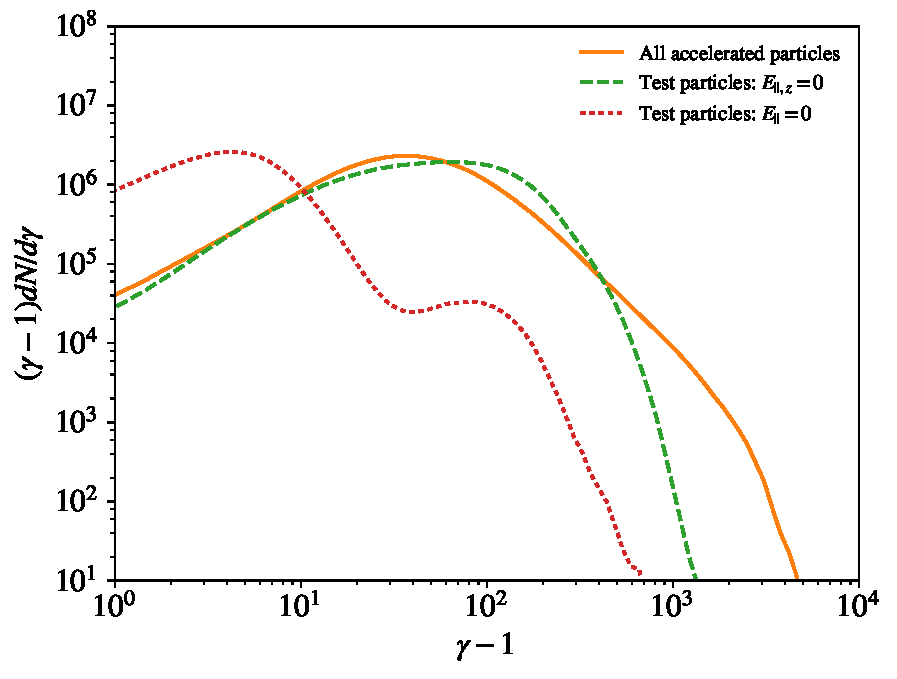
\includegraphics[width=\linewidth]{bguide3_testspec.pdf}
\caption{Spectra of different populations of particles in the triggered $B_{g}=0.3B_{0}$ simulation.  The regular particle spectrum is shown in orange, the solid line corresponds to the spectrum of particles throughout the entire simulation domain while the dash-dot line shows the spectrum from the reconnection region.  The green dashed line shows the spectrum of test particles that do not experience parallel electric fields in the z-direction and the dotted red line shows the spectrum of particles that do not experience any parallel electric fields.  The spectra for test particles are computed only in the reconnection region.}
\label{testprtl_spec}
\end{figure}

\begin{figure}[htp] 
	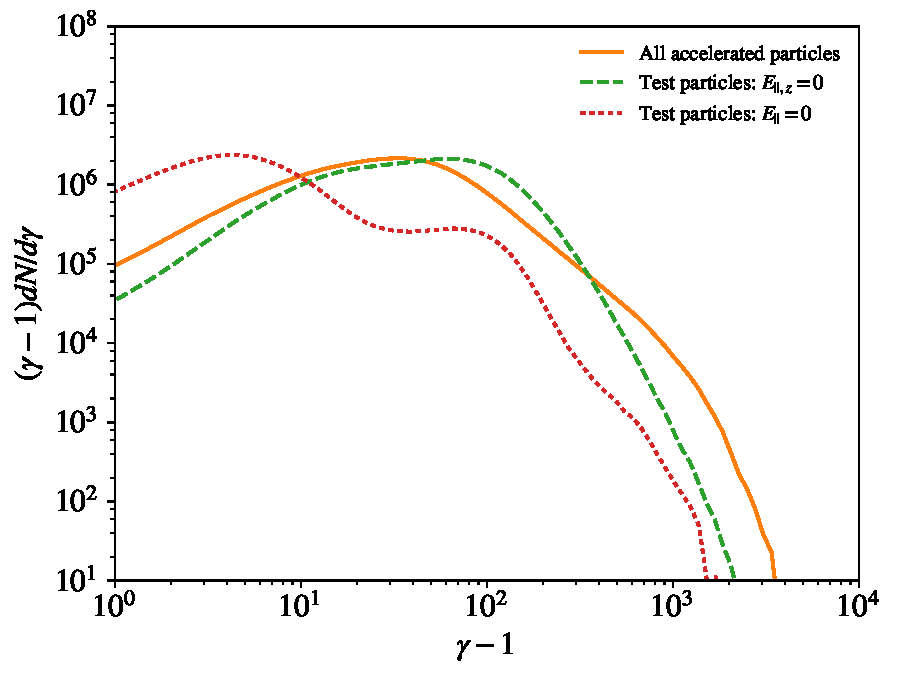
\includegraphics[width=\linewidth]{bguide1_testspec.pdf}
	\caption{Spectra of various populations of test particles from the triggered simulation with $B_{g}=0.1B_{g}$}

	\label{bguide1_testprtl_spec}
\end{figure}




\section{conclusions}
In this work, we have investigated the electron acceleration mechanisms in trans-relativistic reconnection with a set of four PIC simulations.  We include acceleration diagnostics that are calculated on-the-fly for all of the particles so that our results are not affected by the time downsampling of output files, or downsampling the particle number and only looking at a limited selection of particles.  

We vary the number of plasmoids and x-points by varying one parameter related to the simulation setup and one physical parameter.  More specifically, in two of our simulations, we trigger recconection by hand.  This may mimic a thick astrophysical current sheet that gets pinched in a specific location by an external magnetohydrodynamic force.  In the other two simulations, we allow reconnection to evolve spontaneously via the primary tearing mode, this setup mimics an astrophysical situation where a thin current sheet is undisturbed and able to reconnect along its entire length:  in terms of timescales, this requires that the growth rate of the primary tearing instability is faster than any relevant dynamical timescale that would disrupt the current sheet.  In the triggered setups, a primary x-points forms, and results in outflows away from the middle of the box so the only plasmoid mergers that occur are secondary plasmoids that are generated via the secondary tearing mode.  In untriggered setups, the current sheet is pinched at multiple places, resulting in a chain of x-points and plasmoids.  These primary plasmoids will inevitably merge in a hierarchical manner, resulting in numerous large plasmoid mergers towards the end of the simulation.

The physical parameter we vary is the strength of the guide field.  For our values of $\sigma$ and $\beta$, a modest guide field of $B_{g}=0.3B_{0}$ suppresses the secondary tearing mode resulting in a reconnection layer dominated by outflows and a single primary x-point.  For our lower value of $B_{g}=0.1B_{0}$, however, the secondary tearing mode is active, which fractures the current sheet into a series of x-points and plasmoids.

We show that x-points and plasmoid mergers are the dominant sites of electron acceleration due to the strong $E_{||,z}$ that occurs at these locations.  We show this by classifying acceleration episodes of all of our particles as described in Section \ref{acc_mec_def}.  Additionally, we show in Section \ref{E_comps} that the work done by parallel electric fields in the z-direction play a critical role in relativistic electron acceleration.  Finally, in section \ref{test_prtls} we further demonstrate the importance of $E_{||,z}$ by including populations of test particles that are evolved alongside the regular particles in the simulations that do not deposit their currents onto the grid and only feel certain components of $\vec{E}_{||}$.  Using these test particles, we confirm that $E_{||,z}$ is primarily responsible for regulating the high-energy nonthermal tail of the distribution, while the other components of $E_{||}$ are largely associated with bulk heating.

Our results further the understanding of non-thermal electron acceleration in the trans-relativistic regime of reconnection, which is important for potentially understanding the observed X-ray flares from radiatively inefficient accretion flows such as Sgr~A*.   By understanding the electron acceleration mechanisms in this regime, we can more accurately inform efforts to use subgrid models of non-thermal electron acceleration in large-scale MHD simulations of accretion flows.  Ultimately we hope this work will lead to a physically grounded (semi) analytic model for electron acceleration via reconnection.


%\section{Appendix A: Sheet Thickness}\label{thickness_app}
%Explore how the current sheet thickness affects the number of x-points per unit length, and hence energy spectra in an untriggered setup (probably in guide field case, probably in no guide field case, secondary plasmoid formation causes fracturing all over anyways and we have a similar number of x-points per unit length)
\section{Appendix A: Box Size}\label{box_size}
Look at case of triggered vs. untriggered as function of boxsize (with guide field), should see a much steeper dependence of triggered case as opposed to untriggered
\section{Appendix B: Anti-parallel and Low Guide Field Comparison}
In this paper, all of the simulations we use have a non-zero guide field so that we can track the well-defined quantity $W_{||,z}$.  In the case of anti-parallel reconnection, this quantity is not well defined at x-points because the magnetic field is zero at these locations.  In this appendix, we show that our low-guide field ($B_{g}=0.1B_{0}$) results should generalize to the zero guide field case in terms of the acceleration mechanisms.  We show in Figure \ref{bg_spec_compare} the spectra from simulations with identical physical parameters except for a changing guide field, with values of $B_{g}/B_{0}=0, \; 0.1\; $ and $0.3$.  We see that the spectra from $B_{g}/B_{0}=0$ and $B_{g}/B_{0}=0.1$ cases are remarkably similar, with nearly identical power-law slopes.  We additionally examine the typical structures present in each simulation, shown in Figure \ref{bg_flds_compare}.  We see that in the two lowest guide field cases that numerous x-point and plasmoids form, which ultimately result in similar spectra.  In the $B_{g}=0.3B_{0}$ case, however, the structure of the current layer changes dramatically, and these differences are reflected in the spectrum.

\begin{figure}[htp] 
	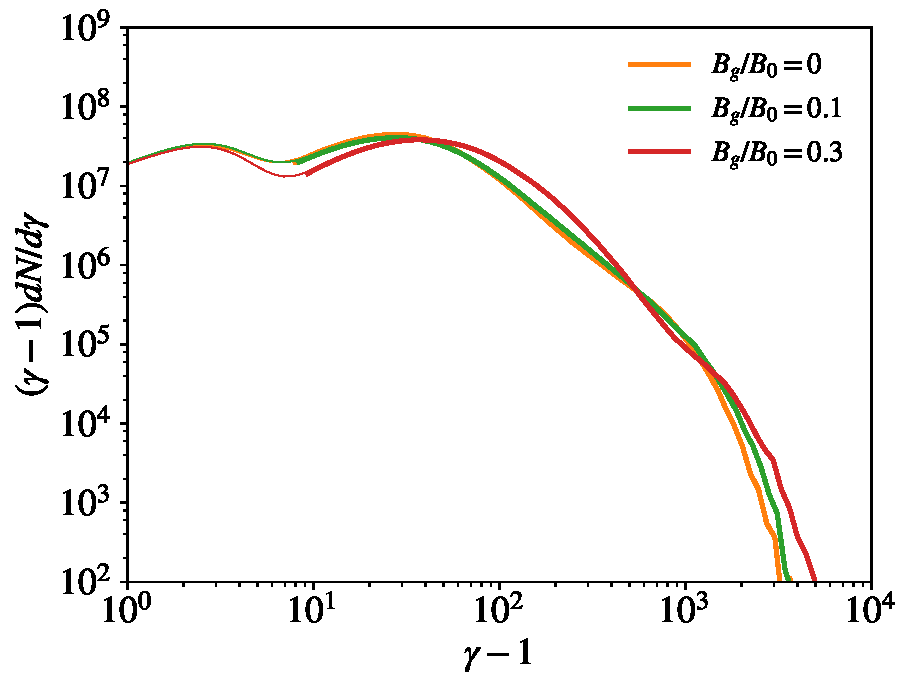
\includegraphics[width=\linewidth]{bg_spec_compare.pdf}
	\caption{Electron energy spectra for simulations with varying guide field.  The zero guide field case is shown in orange and $B_{g}=0.1B_{0}$ and $B_{g}=0.3B_{0}$ are shown with the green and red lines, respectively.  We see that the zero guide field and low guide field spectra are nearly identical, while the higher guide field case shows more overall heating, but a steeper spectrum.}
	\label{bg_spec_compare}
\end{figure}

\begin{figure*}[htp] 
	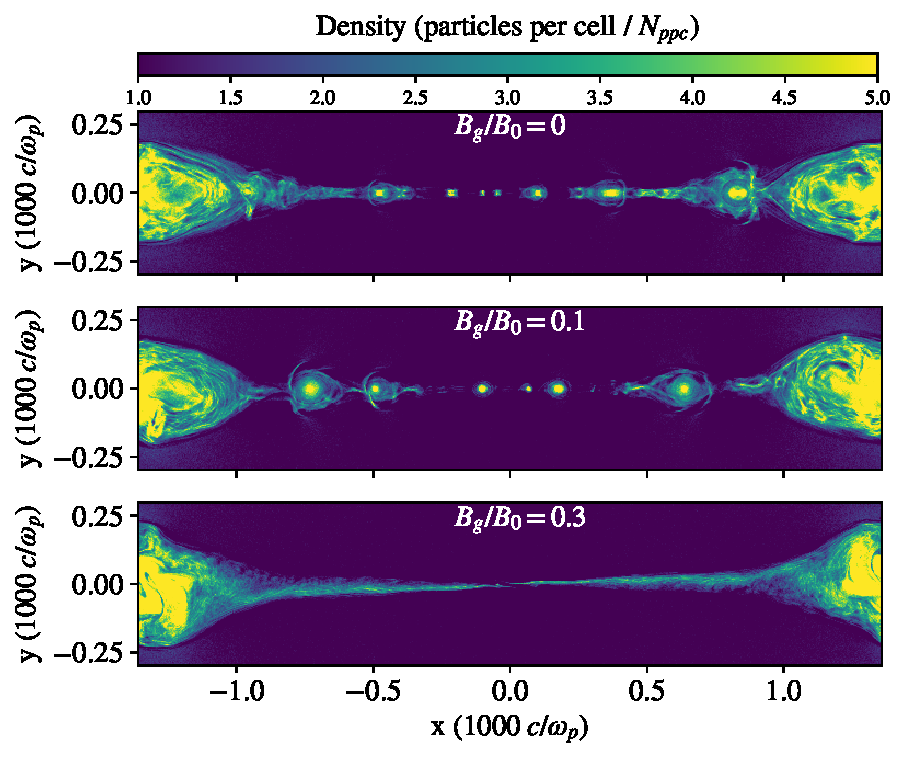
\includegraphics[width=\linewidth]{flds_compare.pdf}
	\caption{Snapshots of density for simulations with varying guide field.  We see that the structures in the purely anti-parallel case (top) and the weak guide field ($B_{g}=0.1$) cases are remarkably similar; plasmoid and x-point formation occur copiously via the secondary tearing mode throughout the reconnection layer.  The higher guide field case (bottom) only shows a single x-point because the secondary tearing mode is suppressed.}
	\label{bg_flds_compare}
\end{figure*}

\FloatBarrier

\bibliography{david_bib}
\bibliographystyle{apj}


\end{document}